\section{Résultats de l'évaluation pratique de l'heuristique}

\subsection{Profil uniforme}

\begin{figure}[h!]
    \begin{subfigure}{\textwidth}
        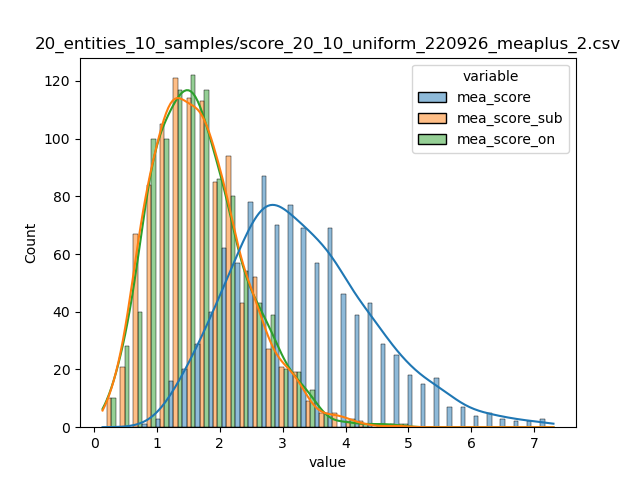
\includegraphics[scale=0.8] {score_20_10_uniform_220926_meaplus_2}
    \end{subfigure}
    \bigskip
    \begin{subfigure}{\textwidth}
        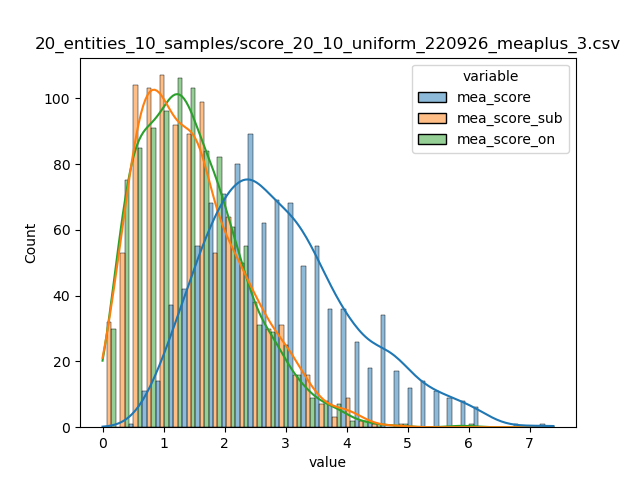
\includegraphics[scale=0.8] {score_20_10_uniform_220926_meaplus_3}
    \end{subfigure}
    \caption{Résultats de 10 ajouts parmi 20 entités avec un prior uniforme discret }
\end{figure}

\begin{figure}[h!]
    \begin{subfigure}{\textwidth}
        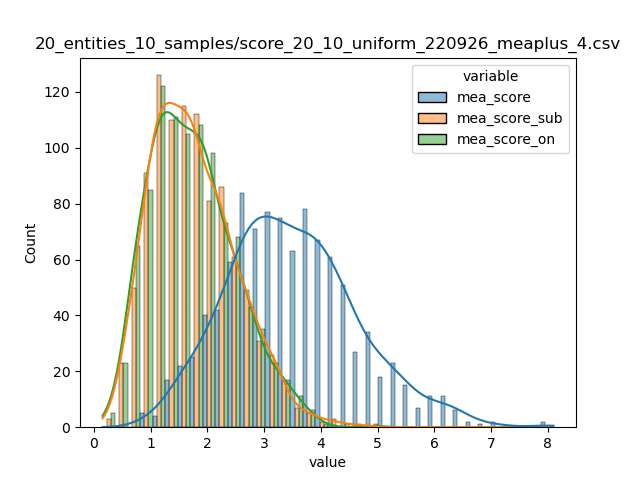
\includegraphics[scale=0.8] {score_20_10_uniform_220926_meaplus_4}
    \end{subfigure}
    \bigskip
    \begin{subfigure}{\textwidth}
        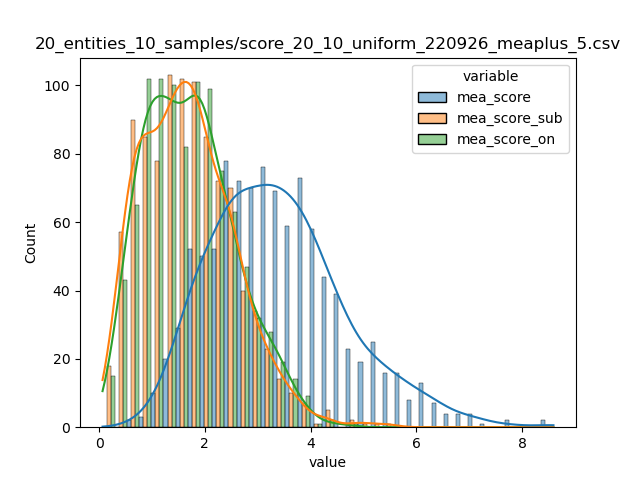
\includegraphics[scale=0.8] {score_20_10_uniform_220926_meaplus_5}
    \end{subfigure}
    \caption{Résultats de 10 ajouts parmi 20 entités avec un prior uniforme discret }
\end{figure}

\pagebreak

\subsection{Profil extrême}


\begin{figure}[h!]
    \begin{subfigure}{\textwidth}
        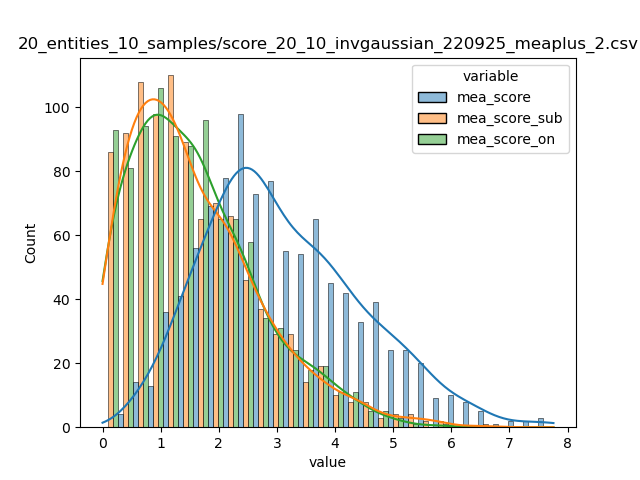
\includegraphics[scale=0.8] {score_20_10_invgaussian_220925_meaplus_2}
    \end{subfigure}
    \bigskip
    \begin{subfigure}{\textwidth}
        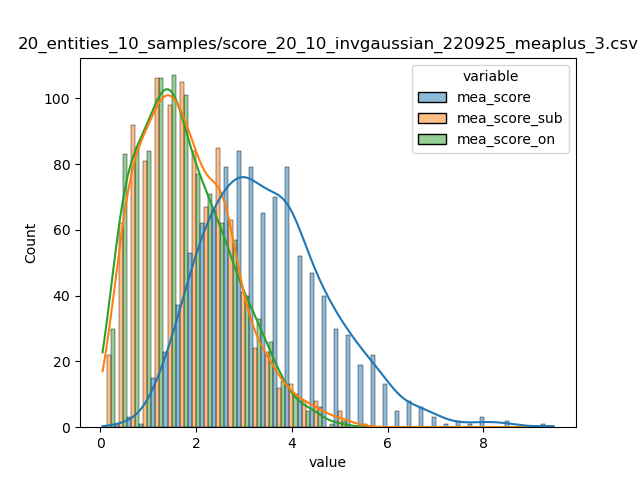
\includegraphics[scale=0.8] {score_20_10_invgaussian_220925_meaplus_3}
    \end{subfigure}
    \caption{Résultats de 10 ajouts parmi 20 entités avec un prior extrême discret }
\end{figure}

\begin{figure}[h!]
    \begin{subfigure}{\textwidth}
        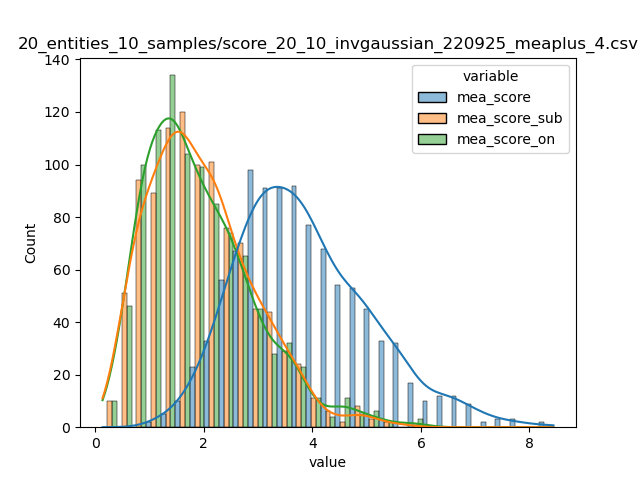
\includegraphics[scale=0.8] {score_20_10_invgaussian_220925_meaplus_4}
    \end{subfigure}
    \bigskip
    \begin{subfigure}{\textwidth}
        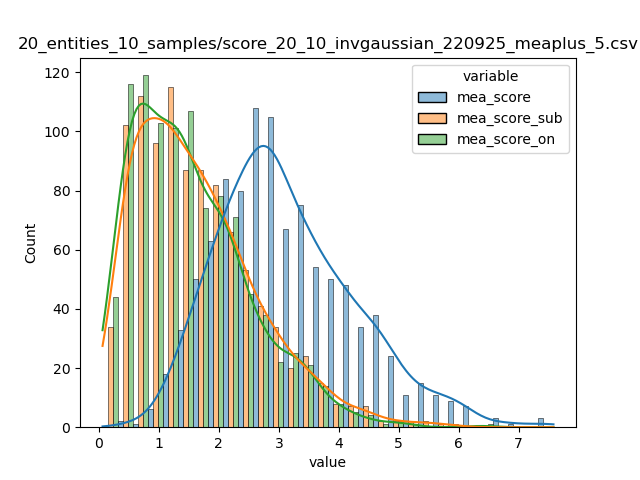
\includegraphics[scale=0.8] {score_20_10_invgaussian_220925_meaplus_5}
    \end{subfigure}
    \caption{Résultats de 10 ajouts parmi 20 entités avec un prior extrême discret }
\end{figure}


\pagebreak

\subsection{Profil gaussien discret}

\begin{figure}[h!]
    \begin{subfigure}{\textwidth}
        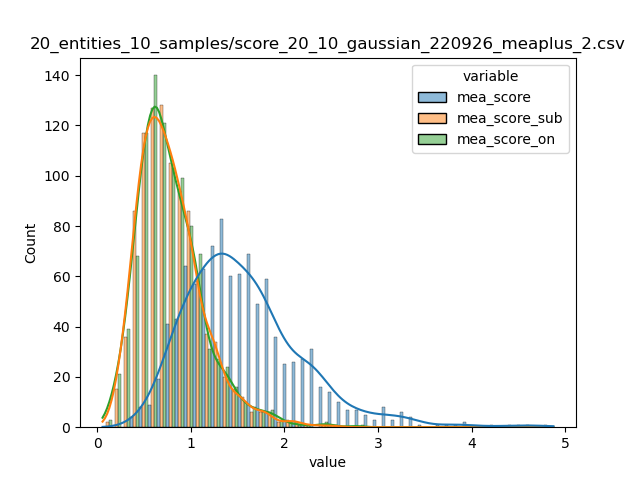
\includegraphics[scale=0.8] {score_20_10_gaussian_220926_meaplus_2}
    \end{subfigure}
    \bigskip
    \begin{subfigure}{\textwidth}
        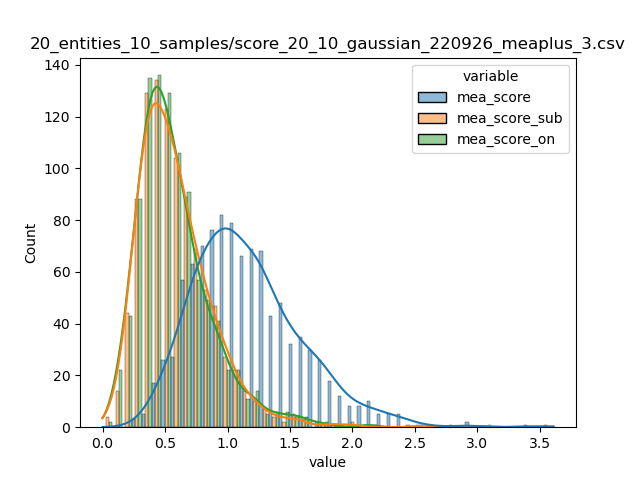
\includegraphics[scale=0.8] {score_20_10_gaussian_220926_meaplus_3}
    \end{subfigure}
    \caption{Résultats de 10 ajouts parmi 20 entités avec un prior gaussien discret }
\end{figure}


\begin{figure}[h!]
    \begin{subfigure}{\textwidth}
        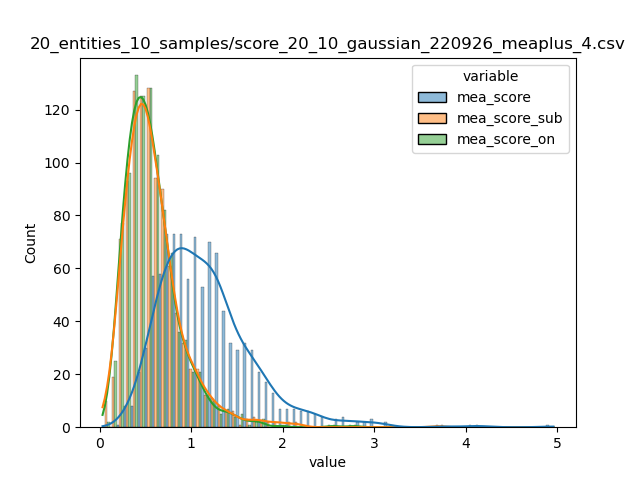
\includegraphics[scale=0.8] {score_20_10_gaussian_220926_meaplus_4}
    \end{subfigure}
    \bigskip
    \begin{subfigure}{\textwidth}
        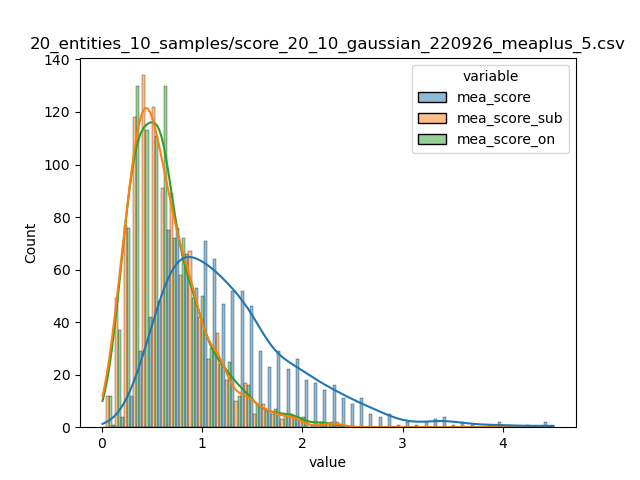
\includegraphics[scale=0.8] {score_20_10_gaussian_220926_meaplus_5}
    \end{subfigure}
    \caption{Résultats de 10 ajouts parmi 20 entités avec un prior gaussien discret }
\end{figure}



